\documentclass[a4paper, 12pt]{article}
\usepackage[utf8]{inputenc}
\usepackage[T1,T2A]{fontenc}
\usepackage[a4paper, top=2cm, bottom=2cm, left=1cm, right=1cm, marginparwidth=1.75cm]{geometry}
\usepackage{graphicx}
\usepackage{amsmath}
\usepackage{indentfirst}
\usepackage[english, russian]{babel}
\usepackage[section,above,below]{placeins}
\usepackage[noend]{algorithmic}
\usepackage{amssymb}
\usepackage{amsfonts}
\usepackage{pdfpages}
\usepackage{xcolor}
\usepackage{hyperref}

\begin{document}

\tableofcontents

\newpage
\section{Методы кластерного анализа}
\textbf{Главное назначение кластерного анализа} --- разбиение множества исследуемых объектов и признаков на однородные в соотвествующем понимании группы (кластеры). Это значит, что \textit{решается задача классификации данных и выявления в ней соответствующей структуры}.

\textbf{Достоинство кластерного анализа} в том, что он позволяет производить разбиение объектов по целому набору признаков, вдобавок не накладывая ограничения на вид рассматриваемых объектов.

\textbf{Задача кластерного анализа} в том, чтобы на основании данных из множества $X$ разбить множество объектов $G$ на $m$ кластеров так, чтобы каждый объект $G_j$ только одному кластеру, а объекты из одного кластера были сходными, покуда объекты из разных кластеров различаются.

\textbf{Методы кластерного анализа} делятся на две группы:
\begin{itemize}
    \item иерархические;
    \item неиерархическиею
\end{itemize}

\section{Иерархические алгоритмы}
Суть иерархической кластеризации состоит в последовательном объединении меньших кластеров в большие (иерархические агломеративные методы) или разделении больших кластеров на меньшие (иерархические дивизимные методы).

Пусть $K_i$ -- $i$-я группа, состоящая из $n$ объектов; $\bar{x}_i$ -- среднее арифметическое векторных наблюдений $K_i$ группы (центр тяжести $i$-й группы); $\rho (K_i,K_j)=\rho{i j}$ --- расстояние между группами $K_i,K_j$.

\textbf{Обобщённая алгомеративная процедура}. На первом шаге каждый объект считается отдельным кластером. На следующем шаге объединяются (в класс) два ближайших объекта, определяются расстояния от этого класса до остальных объектов, размерность матрицы $D$ сокращается на единицу. Такая процедура повтораяется до тех пор, пока все объекты не объединятся в один класс. Если сразу несколько классов имеют наименьшее расстояние, то при объединении выбирают случайную пару (восходящая иерархическая классификация) или объединяют сразу все пары (метод ближайшего соседа).

\section{Расстояния между кластерами}

{\it Возможные расстояния}:
\begin{enumerate}
    \item \textbf{Расстояние "ближайшего соседа"} (одиночная связь): $$\rho_{\min}(K_i,K_j)=\min_{x_i \in K_i, x_j \in K_j} \rho (x_i,x_j).$$ Равно расстоянию между самыми ближними объектами кластеров.
    \item \textbf{Расстояние "дальнего соседа"} (полная связь):$$\rho_{\max}(K_i,K_j)=\max_{x_i \in K_i, x_j \in K_j} \rho (x_i,x_j).$$ Равно расстоянию между самыми дальними объектами кластеров.
    \item \textbf{Невзвешенное попарное среднее}: $$\rho_{\text{mean}}(K_i,K_j)=\text{mean}_{x_i \in K_i, x_j \in K_j} \rho (x_i,x_j).$$ Равно среднему между всеми парами расстояний.
    \item \textbf{Взвешенное попарное среднее}: $$\rho_{\text{mean2}}(K_i,K_j)=\text{mean}_{x_i \in K_i, x_j \in K_j} \rho (k_1 \cdot x_i,k_2 \cdot x_j) = \text{mean}_{x_i \in K_i, x_j \in K_j} \dfrac{k_1 x_i + k_2 x_j}{k_1+k_2}.$$ Равно среднему между всеми парами расстояний с учетом весов $k_1,k_2$, равных ёмкости кластеров.
    \item \textbf{Незвешенный центроидный метод}: расстояние между кластерами равно расстоянию между их центрами тяжести, где центр тяжести есть среднее арифметическое всех объектов в кластере: $$x_c = \dfrac{\sum_{i=1}^k 1 \cdot x_i}{k}= \text{mean}_{x_i \in K_i} (x_i)$$
    \item \textbf{Взвешенный центроидный метод}. Как я понял, это расстояние между центрами, но с учетом весов, как в пункте 4. Но вообще начиная с пункта 4 нигде нет формул, так что не факт, что они у меня правильные.
    \item \textbf{Метод Варда}. Целевой функцией является внутригрупповая сумма квадратов: $$\text{SS}=\sum_i \sum_{x_j \in K_i} \rho(x_j,x_i),$$
    где сумма берётся по всем кластерам, $x_i$ -- среднее по кластеру $K_i$. Объединение в кластеры на каждой итерации происходит так, чтобы увеличение этой функции было минимальным.
\end{enumerate}

\section{Процедуры эталонного типа}
Наряду с иерархическими методами кластеризации существуют итеративные ($k$-средних), суть которых заключается в следующем (возможны модификации):
\begin{enumerate}
    \item Среди объектов $x_i$ некоторым образом выбираются $k$ штук -- центры будущих кластеров.
    \item Объекты, не отнесённые к какому-либо кластеру, приписываются тому кластеру, до которого будет наименьшее расстрояние.
    \item Центры кластеров пересчитываются.
    \item Для всех точек пересматривается их принадлежность к кластеру.
    \item Пункты 3-4 повторяются, пока точки могут менять принадлежность.
\end{enumerate}
На этом сайте хорошо показано, как работает метод $k$-средних: \url{https://www.naftaliharris.com/blog/visualizing-k-means-clustering/}

\section{Методика дискриминантного анализа}
Основной целью дискриминации является нахождение такой линейной комбинации переменных (дискриминантных переменных), которая бы оптимально разделила рассматриваемые группы. Линейная функция:
\begin{equation}
    d_{k m}=\beta_0 + \sum_{i=1}^p \beta_i x_{i k m}, m=1,\dots, n
\end{equation}
называется \textbf{канонической дискриминантной функцией}  с неизвестными коэффициентами. Здесь $d$ -- значение  дискриминантной функции для $m$-го объекта в группе $k$. С геометрической точки зрения дискриминантные функции определяют гиперповерхности в $p$-мерном пространстве. В частном случае при $p = 2$ она является прямой, а при $p = 3$ – плоскостью. 

Коэффициенты  первой канонической дискриминантной функции выбираются таким образом, чтобы центроиды различных групп как можно больше отличались друг от друга. Коэффициенты второй группы выбираются также, но при этом налагается дополнительное условие, чтобы значения второй функции были некоррелированы со значениями первой. Аналогично определяются и другие функции. Если число групп равно $g$, то число канонических дискриминантных функций будет на единицу меньше числа групп. Однако по многим причинам практического характера полезно иметь одну, две или же три дискриминантных функций. Тогда графическое изображение объектов будет представлено в одно-, двух- и трехмерных пространствах. Такое представление особенно полезно в случае, когда число дискриминантных переменных $p$ велико по сравнению с числом групп $g$.

\textbf{Рассмотрим этапы ДА более подробно}
На первом этапе проведения ДА изучаются межгрупповые различия и ищутся ответы на следующие вопросы: возможно ли, используя заданный набор дискриминантных переменных,отличить одну группу от другой; насколько хорошо эти переменные позволяют провести различение; какие из них наиболее информативны. Одним из способов отбора информативных дискриминантных переменных является пошаговый дискриминантный анализ. Логика пошагового ДА такова: вначале определяется та переменная, для которой средние значения в априорно заданных группах "наиболее различны". На каждом следующем шаге рассматриваются условные распределения оставшихся переменных и определяется та, для которой средние значения в группах «наиболее различны». Процесс завершается, когда ни одна из оставшихся переменных не вносит значимого вклада в различение групп (статистика Уилкса, расстояние Махаланобиса и др.). Процедура пошагового ДА предполагает также проверку (в начале каждого шага) всех дискриминантных переменных на соответствие двум условиям: необходимой точности вычисления (толерантности) и превышению заданного уровня различения (с этой целью используют статистики F-ввода и F-исключения). Статистика F-ввода оценивает улучшение различения благодаря использованию данной переменной по сравнению с различением, достигнутым с помощью уже отобранных переменных. Статистика F-исключения определяет значимость ухудшения различения после удаления переменной из списка уже отобранных переменных. На заключительном шаге статистика F-исключения может быть использована для оценки дискриминантных возможностей отобранных переменных. Переменная с наибольшим значение F-исключения дает наибольший вклад в различение, достигнутое посредством других переменных.

На втором этапе проведения ДА отобранное подмножество наиболее информативных переменных используется для вычисления дискриминантных функций. Исследователь получает одну или несколько дискриминантных функций.

Далее определяется все ли вычисленные канонические дискриминантные функции полезны для описания межгрупповых различий. С этой целью используется собственное значение и относительное процентное содержание вычисленных функций (\% объясненной дисперсии), коэффициент канонической корреляции, а также тест равенства средних значений канонических дискриминантных функций в группах. На относительный вклад отдельных дискриминантных переменных в значение каждой дискриминантной функции указывают стандартизированные коэффициенты. Соответственно, чем больше стандартизированный коэффициент, тем больше вклад переменной. Самым лучшим показателем информативности отобранных дискриминантных переменных и полезности применения дискриминантной функции для интерпретации межгрупповых различий является, конечно, процент правильно распознанных объектов с использованием вычисленных дискриминантных функций (классификация с учителем). Число правильно распознанных новых объектов (как в целом, так и по отдельным группам) свидетельствует о соответствии дискриминантной модели эмпирическим данным.

\section{Что характеризует Лямбда Уилкса?}
\textbf{Лямбда Уилкса} — это отношение меры внутригрупповой изменчивости к мере общей изменчивости. Внутригрупповая изменчивость — часть общей, и это означает, что лямбда Уилкса может принимать значения от 0 (группы полностью однородны) до 1 (разделение объектов на группы не приводит к тому, что внутригрупповая изменчивость оказывается меньше общей). Итого, чем меньшее значение имеет лямбда Уилкса, тем лучшим оказывается разделение на группы при дискриминантном анализе.

\section{Что показывают квадраты расстояний Махаланобиса?}
Выбор функций расстояния между объектами для классификации является наиболее очевидным способом введения меры сходства для векторов объектов, которые интерпретируются как точки в евклидовом пространстве. В качестве ме-ры сходства можно использовать евклидово расстояние между объектами. Чем меньше расстояние между объектами, тем больше сходство. Однако в тех случаях, когда переменные коррелированы, измерены в разных единицах и имеют раз-личные стандартные отклонения, трудно четко определить понятие «расстояния». В этом случае полезнее применить не евклидовое расстояние, а \textbf{выборочное расстояние Махаланобиса } 
 \begin{equation}
     D^2({\bf x}/G_k)=(n-g)\cdot ({\bf x}-\bar{\bf x}_k)^T {\bf W}^{-1} ({\bf x}-\bar{\bf x}_k), k=1,\dots,g ,
 \end{equation}
 где \textbf{x} представляет объект с $р$ переменными, $\bar{\bf x}_k$ --- вектор средних для переменных $k$-й группы объектов. Если вместо \textbf{W}   использовать оценку внутригрупповой ковариационной матрицы  
\begin{equation}
    {\bf \Sigma}={\bf W}/(n-g),
\end{equation}
то получим стандартную запись выборочного расстояния Махаланобиса
\begin{equation}
    D^2({\bf x}/G_k)= ({\bf x}-\bar{\bf x}_k)^T {\bf \Sigma}^{-1} ({\bf x}-\bar{\bf x}_k), k=1,\dots,g
\end{equation}
При использовании функции расстояния, объект относят к той группе, для которой расстояние  $D^2$ наименьшее.

\textbf{Расстояние Махаланобиса является мерой расстояния между двумя точками в пространстве, определяемом двумя и более коррелированными переменными}. 


\section{Какое максимальное число канонических дискриминантных функций допустимо в дискриминантном анализе?}
\textit{Общее число дискриминантных функций не превышает числа дискриминантных переменных и, по крайней мере, на единицу меньше числа групп}. Степень разделения выборочных групп зависит от величины собственных чисел: чем больше собственное число, тем сильнее разделение. Наибольшей разделительной способностью обладает первая дискриминантная функция, соответствующая наибольшему собственному числу $\lambda_1$ , вторая обеспечивает максимальное различение после первой и т. д. 

\textbf{Остаточная дискриминация}. Так как дискриминантные функции находятся по выборочным данным, они нуждаются в проверке статистической значимости. Для проверки этой значимости можно воспользоваться критерием, аналогичным дисперсионному критерию в методе главных компонент. Этот критерий оценивает остаточную дискриминантную способность, под которой понимается способность различать группы, если при этом исключить информацию, полученную с помощью ранее вычисленных функций. Если остаточная дискриминация мала, то не имеет смысла дальнейшее вычисление очередной дискриминантной функции. Полученная статистика носит название $\Lambda$-статистики Уилкса и вычисляется по формуле:
 \begin{equation}
    \Lambda = \prod_{i=k+1}^g \dfrac{1}{1+\lambda_i}, 
 \end{equation}
где $k$ -- число вычисленных функций. Чем меньше эта статистика, тем значимее соответствующая дискриминантная функция. Величина
\begin{equation}
    \chi^2=-\left(n-1-\dfrac{p+g}{2}  \right) \ln \Lambda_k, k=0,1,\dots,g-1
\end{equation}
имеет хи-квадрат распределение с  $(p-k)(g-k-1)$ степенями свободы. 

Вычисления проводим в следующем порядке.
\begin{enumerate}
    \item Находим значение критерия  $\chi^2$ при $k = 0$. Значимость критерия подтверждает существование различий между группами. Кроме того, это доказывает, что первая дискриминантная функция значима и имеет смысл ее вычислять.
    \item Определяем первую дискриминантную функцию, и проверяем значимость критерия при $k = 1$. Если критерий значим, то вычисляем вторую дискриминантную функцию и продолжаем процесс до тех пор, пока не будет исчерпана вся значимая информация.
\end{enumerate}

\section{Какую информацию дают стандартизованные и структурные коэффициенты дискриминантной функции?}
 \textbf{Стандартизованные коэффициенты}  -- это то же самое, что и нестандартизованные, но полученные по стандартизованным начальным данным. \textit{Стандартизованные коэффициенты полезно применять для уменьшения размерности исходного признакового пространства переменных: если абсолютная величина коэффициента для данной переменной для всех дискриминантных функций мала, то эту переменную можно исключить, тем самым сократив число переменных.} 

\textbf{Структурные коэффициенты}  определяются коэффициентами взаимной корреляции между отдельными переменными и дискриминантной функцией. Если относительно некоторой переменной абсолютная величина коэффициента велика, то вся информация о дискриминантной функции заключена в этой переменной. 

Структурные коэффициенты по своей информативности несколько отличаются от стандартизованных коэффициен-тов. \textit{Стандартизованные коэффициенты показывают вклад переменных в значение дискриминантной функции}. Если две переменные сильно коррелированы, то их стандартизованные коэффициенты могут быть меньше по сравнению с теми случаями, когда используется только одна из этих переменных. Такое распределение величины стандартизованного коэффициента объясняется тем, что при их вычислении учитывается влияние всех переменных. \textit{Структурные же коэффициенты являются парными корреляциями и на них не влияют взаимные зависимости прочих переменных}.

\section{Опишите процедуру отбора переменных с помощью стандартизованных и структурных коэффициентов}
Никакой инфы про эту процедуру "отбора переменных с помощью стандартизованных и структурных коэффициентов" я не нашёл. Структурные коэффициенты вообще показывают корреляцию между переменной и дискриминантной функцией, что позволяет {\it интепретировать} результаты, а не отбирать переменные. Можете сами попробовать поискать что-то про это в копии её методички: \url{http://masters.donntu.org/2005/kita/kapustina/library/discr_an.htm}.

{\it Про стандартизованные коэффициенты есть такая инфа}: "В рамках алгоритмического подхода список информативных
переменных формируется автоматически в соответствии с тем
или иным алгоритмом пошагового дискриминантного анализа.
Предусмотрены два его варианта: «Forward stepwise» и
«Backward stepwise» –- метод последовательного пополнения и
метод последовательного исключения списка информативных
признаков. В первом случае выбирается переменная, вносящая
наибольший вклад в межгрупповые различия, и далее к ней на
каждом шаге анализа присоединятся другие информативные переменные. Метод исключения основан на альтернативной процедуре: из полного списка признаков на каждом шаге анализа последовательно исключаются малозначимые переменные." При этом величина вклада переменной в различия определяется как раз величиной стандартизованного коэффициента.

\textbf{Пошаговый дискриминантный анализ}.

Вероятно, наиболее общим применением дискриминантного анализа является включение в исследование многих переменных с целью определения тех из них, которые наилучшим образом разделяют совокупности между собой.

\textbf{Модель}. Другими словами, вы хотите построить "модель", позволяющую лучше всего предсказать, к какой совокупности будет принадлежать тот или иной образец. В следующем рассуждении термин "в модели" будет использоваться для того, чтобы обозначать переменные, используемые в предсказании принадлежности к совокупности; о неиспользуемых для этого переменных будем говорить, что они "вне модели".

\textbf{Пошаговый анализ с включением}. В пошаговом анализе дискриминантных функций модель дискриминации строится по шагам. Точнее, на каждом шаге просматриваются все переменные и находится та из них, которая вносит наибольший вклад в различие между совокупностями. Эта переменная должна быть включена в модель на данном шаге, и происходит переход к следующему шагу.

\textbf{Пошаговый анализ с исключением}. Можно также двигаться в обратном направлении, в этом случае все переменные будут сначала включены в модель, а затем на каждом шаге будут устраняться переменные, вносящие малый вклад в предсказания. Тогда в качестве результата успешного анализа можно сохранить только "важные" переменные в модели, то есть те переменные, чей вклад в дискриминацию больше остальных.

\section{Какова интерпретация канонического коэффициента корреляции?}
Общее число дискриминантных функций не превышает числа дискриминантных переменных и, по крайней мере, на единицу меньше числа групп. Степень разделения выборочных групп зависит от величины собственных чисел: чем больше собственное число, тем сильнее разделение. Наибольшей разделительной способностью обладает первая дискриминантная функция, соответствующая наибольшему собственному числу $\lambda_i$, вторая обеспечивает максимальное различение после первой и т. д. Различительную способность $i$-й функции оценивают по относительной величине в процентах собственного числа  $\lambda_i$ от суммы всех  $\lambda$.

\textbf{Коэффициент канонической корреляции}. Другой характеристикой, позволяющей оценить полезность дискриминантной функции является коэффициент канонической корреляции  $r_i$. Каноническая корреляция является мерой связи между двумя множествами переменных. Максимальная величина этого коэффициента равна 1. Будем считать, что группы составляют одно множество, а другое множество образуют дискриминантные переменные. Коэффициент канонической корреляции для $i$-й дискриминантной функции определяется формулой: $$r_i = \sqrt{\dfrac{\lambda_i}{1+\lambda_i}}.$$

\textbf{Чем больше величина  $r_i$, тем лучше разделительная способность дискриминантной функции.}

\section{В каком случае учет априорных вероятностей может сильно изменить результаты классификации?}
Априорные вероятности оказывают наибольшее влияние при перекрытии групп и, следовательно, многие объекты с большой вероятностью могут принадлежать ко многим группам. Если группы сильно различаются, то учет априорных вероятностей практически не влияет на результат классификации, поскольку между классами будет находиться очень мало объектов
\section{Методика факторного анализа}

\textbf{Факторный анализ} -- раздел статистического многомерного анализа, объединяющий методы оценки размерности множества наблюдаемых переменных посредством исследования структуры ковариационных или корреляционных матриц.

Факторный анализ (ФА) представляет собой совокупность методов, которые на основе реально существующих связей анализируемых признаков, связей самих наблюдаемых объектов, позволяют выявлять скрытые (неявные, латентные) обобщающие характеристики организационной структуры и механизма развития изучаемых явлений, процессов. Основное предположение факторного анализа заключается в том, что корреляционные связи между большим количеством наблюдаемых переменных можно объяснить существованием меньшего числа гипотетических переменных или факторов, называемых общими скрытыми факторами. Далее их будем называть просто факторами.
Факторный анализ может быть:
\begin{itemize}
    \item разведочным — он осуществляется при исследовании скрытой факторной структуры без предположения о числе факторов и их нагрузках;
    \item конфирматорным, предназначенным для проверки гипотез о числе факторов и их нагрузках.
\end{itemize}

\textbf{Фактор} – латентная переменная, конструируемая таким образом, чтобы можно было объяснить корреляцию между набором некоторых имеющихся переменных.
\textbf{Нагрузка} – корреляция между исходной переменной и фактором.

Общей моделью факторного анализа служит следующая линейная зависимость:
\begin{equation}
    x_i = \sum_{j=1}^m a_{i j} F_j+ b_i U_i + \varepsilon_i, i = 1, \dots, k,
\end{equation}
где $F_j$ -- общие факторы, $x_i$ -- наблюдаемые переменные, $U_i$ -- характерные факторы, $ \varepsilon_i$ -- случайные ошибки.

\begin{figure}[h!]
    \center{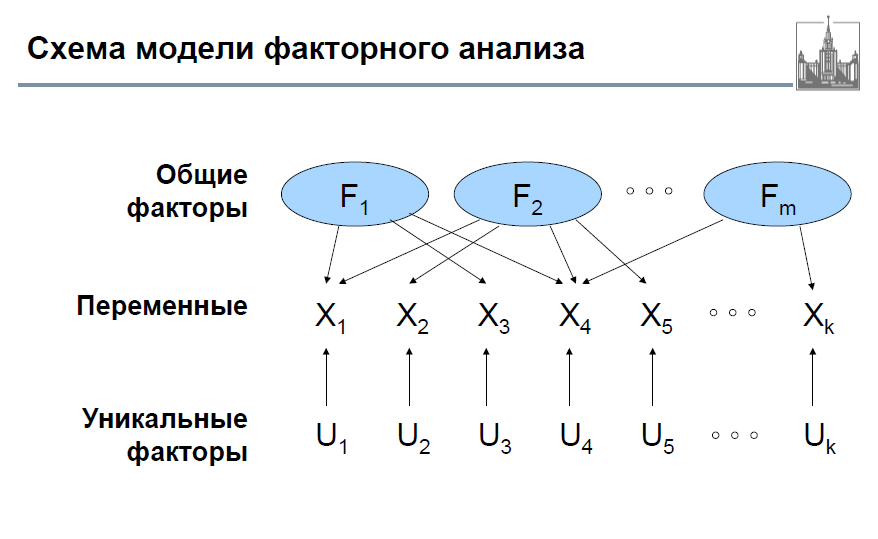
\includegraphics[width=0.9\linewidth]{factors.png}}
    \caption{Схема}
    \label{ris:image}
    \end{figure}

Главными целями факторного анализа являются:
\begin{itemize}
    \item сокращение числа переменных (редукция данных);
    \item определение структуры взаимосвязей между переменными, т.е. классификация переменных.
\end{itemize}
­	
­Практическое выполнение факторного анализа начинается с проверки его условий. В обязательные условия факторного анализа входят:
\begin{itemize}
    \item все признаки должны быть количественными;
    \item число наблюдений должно быть не менее чем в два раза больше числа переменных;
    \item выборка должна быть однородна.
\end{itemize}

Для проведения факторного анализа предлагается методика, включающая в себя следующие этапы:
\begin{enumerate}
    \item сбор исходных статистических данных и подготовка корреляционной (ковариационной) матрицы;
    \item выделение общих скрытых факторов;
    \item вращение факторной структуры;
    \item содержательная интерпретация результатов факторного анализа.
\end{enumerate}

Алгоритмы факторного анализа основываются на использовании редуцированной матрицы парных корреляций (ковариаций).
\textbf{Редуцированная матрица} – это матрица парных коэффициентов корреляции, на главной диагонали которой расположены не единицы (оценки) полной корреляции или оценки полной дисперсии, а их редуцированные, несколько уменьшенные величины – значения оценок общностей. Общность характеризует вклад данного признака в суммарную общность процесса
При этом постулируется, что в результате анализа будет объяснена не вся дисперсия изучаемых признаков (объектов), а ее некоторая часть, обычно большая. Оставшаяся необъясненная часть дисперсии — это характерность, возникающая из-за специфичности наблюдаемых объектов, или ошибок, допускаемых при регистрации явлений, процессов, т.е. ненадежности вводных данных.
	


\section{Суть задачи вращения общих факторов}
Задача вращения общих факторов решается с целью улучшения их {\it интерпретируемости}. Производится попытка достижения простой структуры, в которой каждая переменная характеризуется преобладающим влиянием какого–то одного фактора. Факторные нагрузки могут быть изображены в виде диаграммы рассеяния, на которой каждая переменная представлена точкой. Можно повернуть оси в любом направлении без изменения относительного положения точек. При этом действительные координаты точек, то есть факторные нагрузки, изменяются. 
\begin{figure}[h!]
    \center{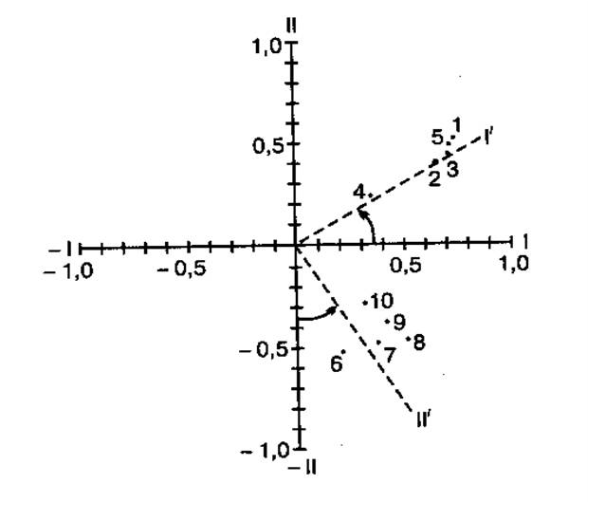
\includegraphics[width=0.5\linewidth]{rotate.png}}
    \caption{Вращение факторов}
    \label{ris:image}
    \end{figure}

Существуют различные методы вращения факторов. Целью этих методов является получение понятной (интерпретируемой) матрицы нагрузок, то есть факторов, которые ясно отмечены высокими нагрузками для некоторых переменных и низкими -- для других. 

{\it Примеры методов вращения}:
\begin{itemize}
    \item­	\textbf{Варимакс}. Ортогональный метод вращения, минимизирующий число переменных с высокими нагрузками на каждый фактор. 
    \item ­	\textbf{Метод косоугольного (неортогонального) вращения}. Самое косоугольное решение соответствует дельте, равной 0 (по умолчанию). По мере того, как дельта отклоняется в отрицательную сторону, факторы становятся более ортогональными.
    \item ­	\textbf{Квартимакс}. Метод вращения, который минимизирует число факторов, необходимых для объяснения каждой переменной.
    \item ­	\textbf{Эквимакс}. Метод вращения, объединяющий методы варимакс, упрощающий факторы, и квартимакс, упрощающий переменные. Минимизируется число переменных с большими факторными нагрузками и число факторов, требуемых для объяснения переменной.
    \item ­	\textbf{Промакс-вращение}. Косоугольное вращение в предположении, что факторы могут коррелировать между собой. Оно производится быстрее, чем вращение типа косоугольного вращения, поэтому оно полезно для больших наборов данных.
\end{itemize}

\textbf{Примечание}. КОСОУГОЛЬНОЕ ВРАЩЕНИЕ --- такая трансформация факторного пространства, которая предполагает возможность проведения факторных осей под углами друг к другу, отличающимися от 90 градусов (от ортогональности)

\section{Критерий Кайзера}
\textbf{Критерий Кайзера или критерий собственных чисел}: отбираются только факторы с собственными значениями равными или большими 1. Это означает, что если фактор не выделяет дисперсию, эквивалентную, по крайней мере, дисперсии одной переменной, то он опускается. Этот критерий предложен Кайзером (Kaiser, 1960), и является, вероятно, наиболее широко используемым.
\section{Критерий Каменистой осыпи}
\textbf{Критерий каменистой осыпи} является графическим методом, где собственные значения представляются в виде простого графика. \textit{Необходимо найти такое место на графике, где убывание собственных значений слева направо максимально замедляется.}  
Справа от этой точки находится, по-видимому, только "факторная осыпь"; "осыпь" --- это геологический термин для обломков, которые скапливаются в нижней части каменистого склона.
 
\begin{figure}[h!]
    \center{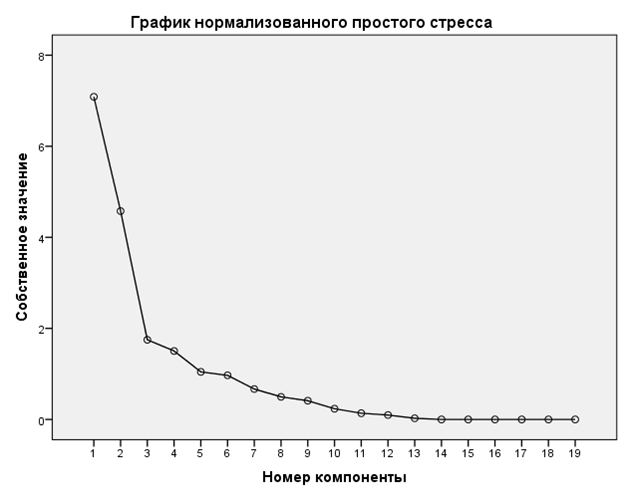
\includegraphics[width=0.7\linewidth]{osp.png}}
    \caption{График собственных значений общих факторов}
    \label{ris:image}
    \end{figure}

По графику видно, что только три фактора влияют на анализ. Их и необходимо оставить. Но иногда такое количество факторов не покрывает необходимый процент выборки и тогда берется больше факторов.
\section{Метод главных компонент}

\textbf{Метод главных компонент} --- это технология многомерного статистического анализа, используемая для сокращения размерности пространства признаков с минимальной потерей полезной информации, которая представляет собой ортогональное линейное преобразование, которое отображает данные из исходного пространства признаков в новое пространство меньшей размерности.

При этом первая ось новой системы координат строится таким образом, чтобы дисперсия данных вдоль неё была бы максимальна. Вторая ось строится ортогонально первой так, чтобы дисперсия данных вдоль неё, была бы максимальной их оставшихся возможных и т.д. Первая ось называется первой главной компонентой, вторая -- второй и т. д.
 
\begin{figure}[h!]
    \center{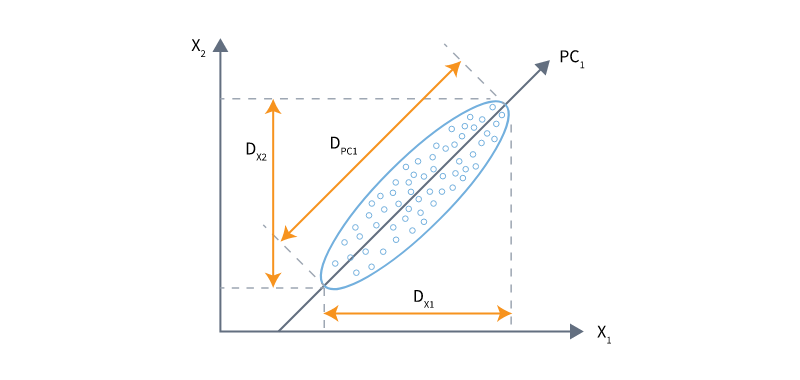
\includegraphics[width=0.7\linewidth]{prc.png}}
    \label{ris:image}
    \end{figure}

На рисунке показано снижение размерности исходного 2-мерного пространства (X1,X2) с помощью метода главных компонент до 1-мерного. Первая главная компонента PC1 ориентирована вдоль направления наибольшей вытянутости эллипсоида рассеяния точек объектов исходного набора данных в пространстве признаков, т.е. с ней связана наибольшая дисперсия.

На рисунке, также, несложно увидеть, что проекция дисперсии данных на ось первой главной компоненты DPC1, больше, чем её проекции на исходные оси DX1 и DX2, но меньше их суммы. Т.е. с помощью первой главной компоненты выразить всю дисперсию данных не удалось. Поэтому строят вторую, третью и т.д. главные компоненты, пока они суммарно не отразят (почти) всю дисперсию.

Смысл метода заключается в том, что с каждой главной компонентой связана определённая доля общей дисперсии исходного набора данных (её называют нагрузкой). В свою очередь, дисперсия, являющаяся мерой изменчивости данных, может отражать уровень их информативности.

Задача метода главных компонент заключается в том, чтобы построить новое пространство признаков меньшей размерности, дисперсия между осями которой будет перераспределена так, чтобы максимизировать дисперсию по каждой из них. Для этого выполняется последовательность следующих действий:
\begin{enumerate}
    \item Вычисляется общая дисперсия исходного пространства признаков. Это нельзя сделать простым суммированием дисперсий по каждой переменной, поскольку они, в большинстве случаев, не являются независимыми. Поэтому суммировать нужно взаимные дисперсии переменных, которые определяются из ковариационной матрицы.
    \item Вычисляются собственные векторы и собственные значения ковариационной матрицы, определяющие направления главных компонент и величину связанной с ними дисперсии.
    \item Производится снижение размерности. Диагональные элементы ковариационной матрицы показывают дисперсию по исходной системе координат, а её собственные значения -- по новой. Тогда разделив дисперсию, связанную с каждой главной компонентой на сумму дисперсий по всем компонентам, получаем долю дисперсии, связанную с каждой компонентой. После этого отбрасывается столько главных компонент, чтобы доля оставшихся составляла 80-90\%.
\end{enumerate}

Основными ограничениями метода главных компонент являются:
\begin{itemize}
    \item невозможность смысловой интерпретации компонент, поскольку они "вбирают" в себя дисперсию от нескольких исходных переменных;
    \item метод может работать только с непрерывными данными.
\end{itemize}


\end{document}